\chapter{Discussion of Experimental Errors}
\label{Errors}
\section{Resolution of measurement}
The position of a detected particle is known to within a specified distance, which translates into a resolution in the measurement of the opening angle between a pair of particles.
A particle's reconstructed position along a detector's length has an error of $\pm$13 cm.
Due to the detector's 15 cm width, there is also a positional uncertainty of $\pm 7.5$ cm in the direction perpendicular along the detector's length.
The amount of uncertainty in a single two-neutron opening angle measurement is determined from the uncertainties in the positions of each detected neutron.
These position uncertainties are propagated through the formula for the calculation of opening angle, which is
\begin{displaymath}
    \theta_{nn} = \text{arccos}\left(\frac{\vec{v_{1}}^{\,}\cdot\vec{v_{2}}^{\,}}{|\vec{v_{1}}^{\,}||\vec{v_{2}}^{\,}|}\right)
\end{displaymath}
where $\vec{v_{1}}^{\,} = (x_1,y_1,z_1)$ and $\vec{v_{2}}^{\,} = (x_2,y_2,z_2)$ are the detected positions of the two neutrons.
The propagation of error through this formula is achieved by evaluating the following expression
\begin{eqnarray}
\label{eq:propagation}
 \Delta \theta_{nn} & = & \left( \left(\Delta x_1 \frac{\partial \theta}{\partial x_1}\right)^{2} + \left(\Delta y_1 \frac{\partial \theta}{\partial y_1}\right)^{2} + \left(\Delta z_1 \frac{\partial \theta}{\partial z_1}\right)^{2} + \right. \\
 & & \left. + \left(\Delta x_2 \frac{\partial \theta}{\partial x_2}\right)^{2} + \left(\Delta y_2\frac{\partial \theta}{\partial y_2}\right)^{2} + \left(\Delta z_2 \frac{\partial \theta}{\partial z_2}\right)^{2} \right) ^{\frac{1}{2}} \, ,  \nonumber
\end{eqnarray}
where the $\Delta$'s represent the uncertainty in the variable that directly follows each $\Delta$.
The values and uncertainties of all events in a given opening angle bin are fed through Eq. \ref{eq:propagation}, and then the results are averaged.
The result is shown in Fig.~\ref{fig:OpeningAngleRes} and can be interpreted as the opening angle resolution as a function of $\theta_{nn}$.
\begin{figure}[h]
    \centering
    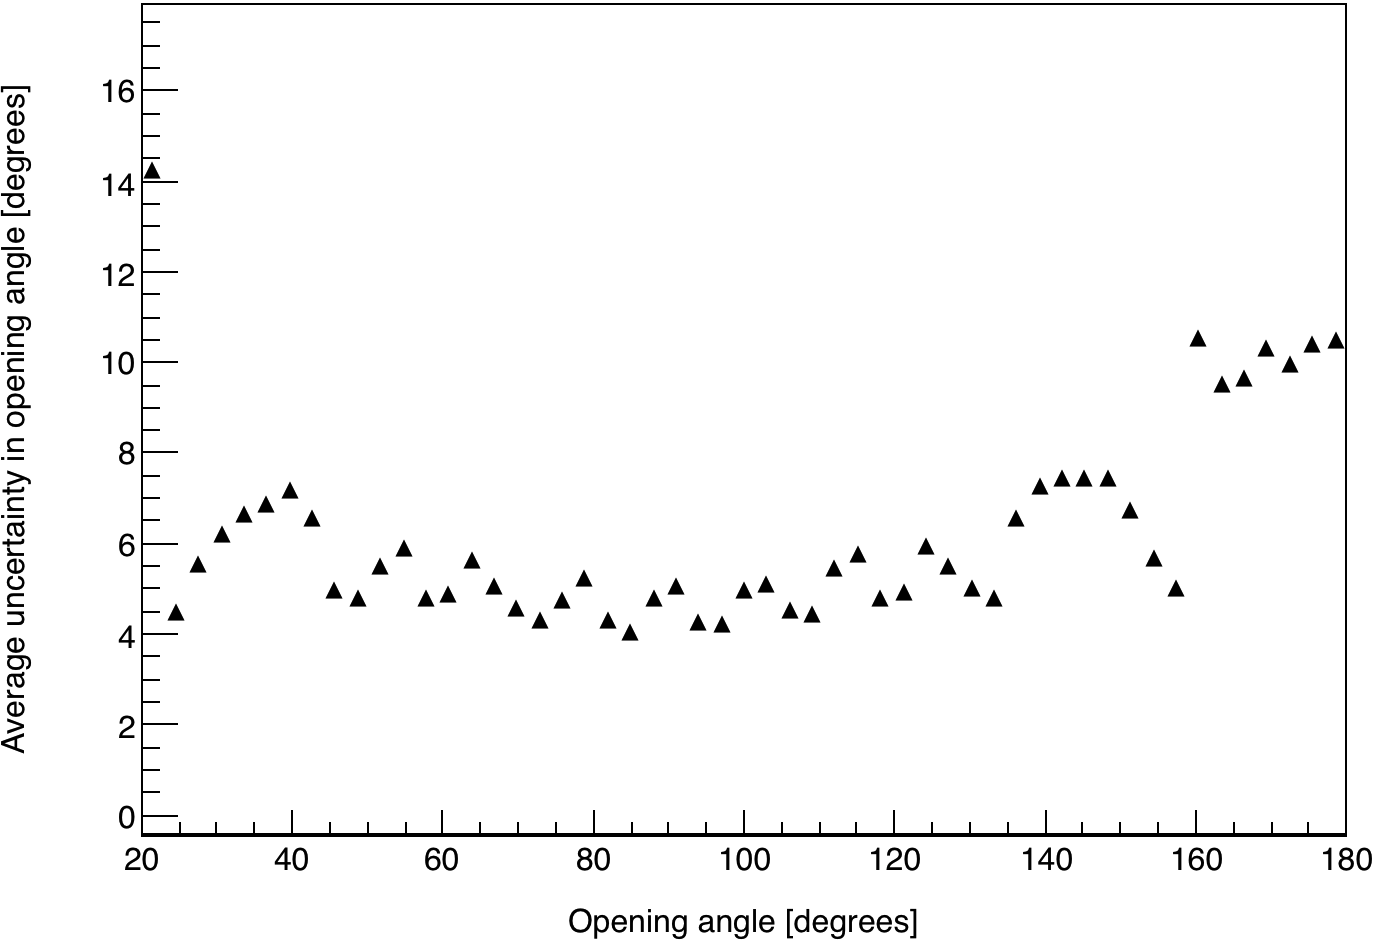
\includegraphics[width = 0.85\textwidth]{Content/Errors/OpeningAngleUncertainty.png}
    \caption{Uncertainties in opening angle determined from the propagation of position uncertainties through the opening angle calculation.
     The uncertainty of a given opening angle measurement depends on which detectors are involved and the position of the particles on the detectors.
     For this reason, the uncertainty of measurements falling within each angle bin is a distribution, so the average uncertainties are plotted here.
    The y-axis can be viewed as a measure of angular resolution in the sense that it represents the smallest angular difference that can be considered statistically significant.
    }
    \label{fig:OpeningAngleRes}
\end{figure}

\section{Counting error}
The uncertainty in the number of observed events is always assumed to be equal to $\sqrt{N}$, as per Poissonian  statistics, where N is the number of observed events.
This value is then propagated through all the analysis procedure using the standard methods for the propagation of error.
The vertical error bars seen in all results are due solely to such counting error.

\FloatBarrier
\section{Detector Cross-talk}
\label{crosstalk}
\textit{Cross-talk} occurs when, after a particle is detected once, the same particle, by any means, causes a detection to be registered in a different detector.
For example, upon detection, a particle may undergo elastic scattering and then travel into a another detector where it is detected again, or it may produce secondary particles that are detected.
The two coincident detections of a cross-talk event are causally correlated, and thus they have the potential to contaminate the signal from correlated fission neutrons.
If both detections occur during the ToF range typical for fission neutrons, then the cross-talk event cannot be distinguished from the detection of two correlated neutrons.

Recent works that measured the two-neutron angular correlations in the spontaneous fission of $^{252}$Cf and $^{240}$Pu~\cite{Pozzi2016,Verbeke2018} addressed this effect by using an MCNP-PoLiMi simulation to estimate and then subtract cross-talk from their measurements.
In this work, the issue of cross-talk is approached differently by employing the use of detector shielding aimed at reducing cross-talk to a negligible rate.
By using shielding to reduce cross-talk, this measurement is less dependent on the details of the models used by MCNP-PoLiMi to simulate neutron transport and detection.
MCNP-PoLoMi simulations are used in this work only to verify that the effect of cross-talk is negligible.
The scintillators used here are much larger than those used in similar works, such as in refs~\cite{Pozzi2016,Verbeke2018}, allowing them to be placed much farther from the fission source without causing extremely low coincidence rates. 
An increase in the distance between the detectors and the fission source makes this measurement less sensitive to angular uncertainty, which is influenced by the uncertainty in the position of a detected particle due to, for example, the scattering of neutrons from detector shielding.
Because of this, larger amounts of shielding can be used without concern of introducing large errors.

The geometry of the neutron detection system makes it kinematically impossible for a neutron to scatter from a proton in one detector--which is the basis for scintillation--and then travel directly into another detector with enough kinetic energy to be detected a second time.
For this reason, upon being detected, a neutron must scatter from one or more intermediate nuclei, such as Pb or C, in order for it to reach a different detector with enough energy to be detected a second time.
This fact follows from the conservation of energy and momentum.
Figure~\ref{fig:CrossTalkExample} illustrates a cross-talk event due to a neutron scattering in a detector's shielding.
In order to be more convinced that such events occur at negligible rates, a detailed MCNP-PoliMi~\cite{MCNP_POLIMI} simulation was performed to model cross-talk.
\begin{figure}
    \centering
    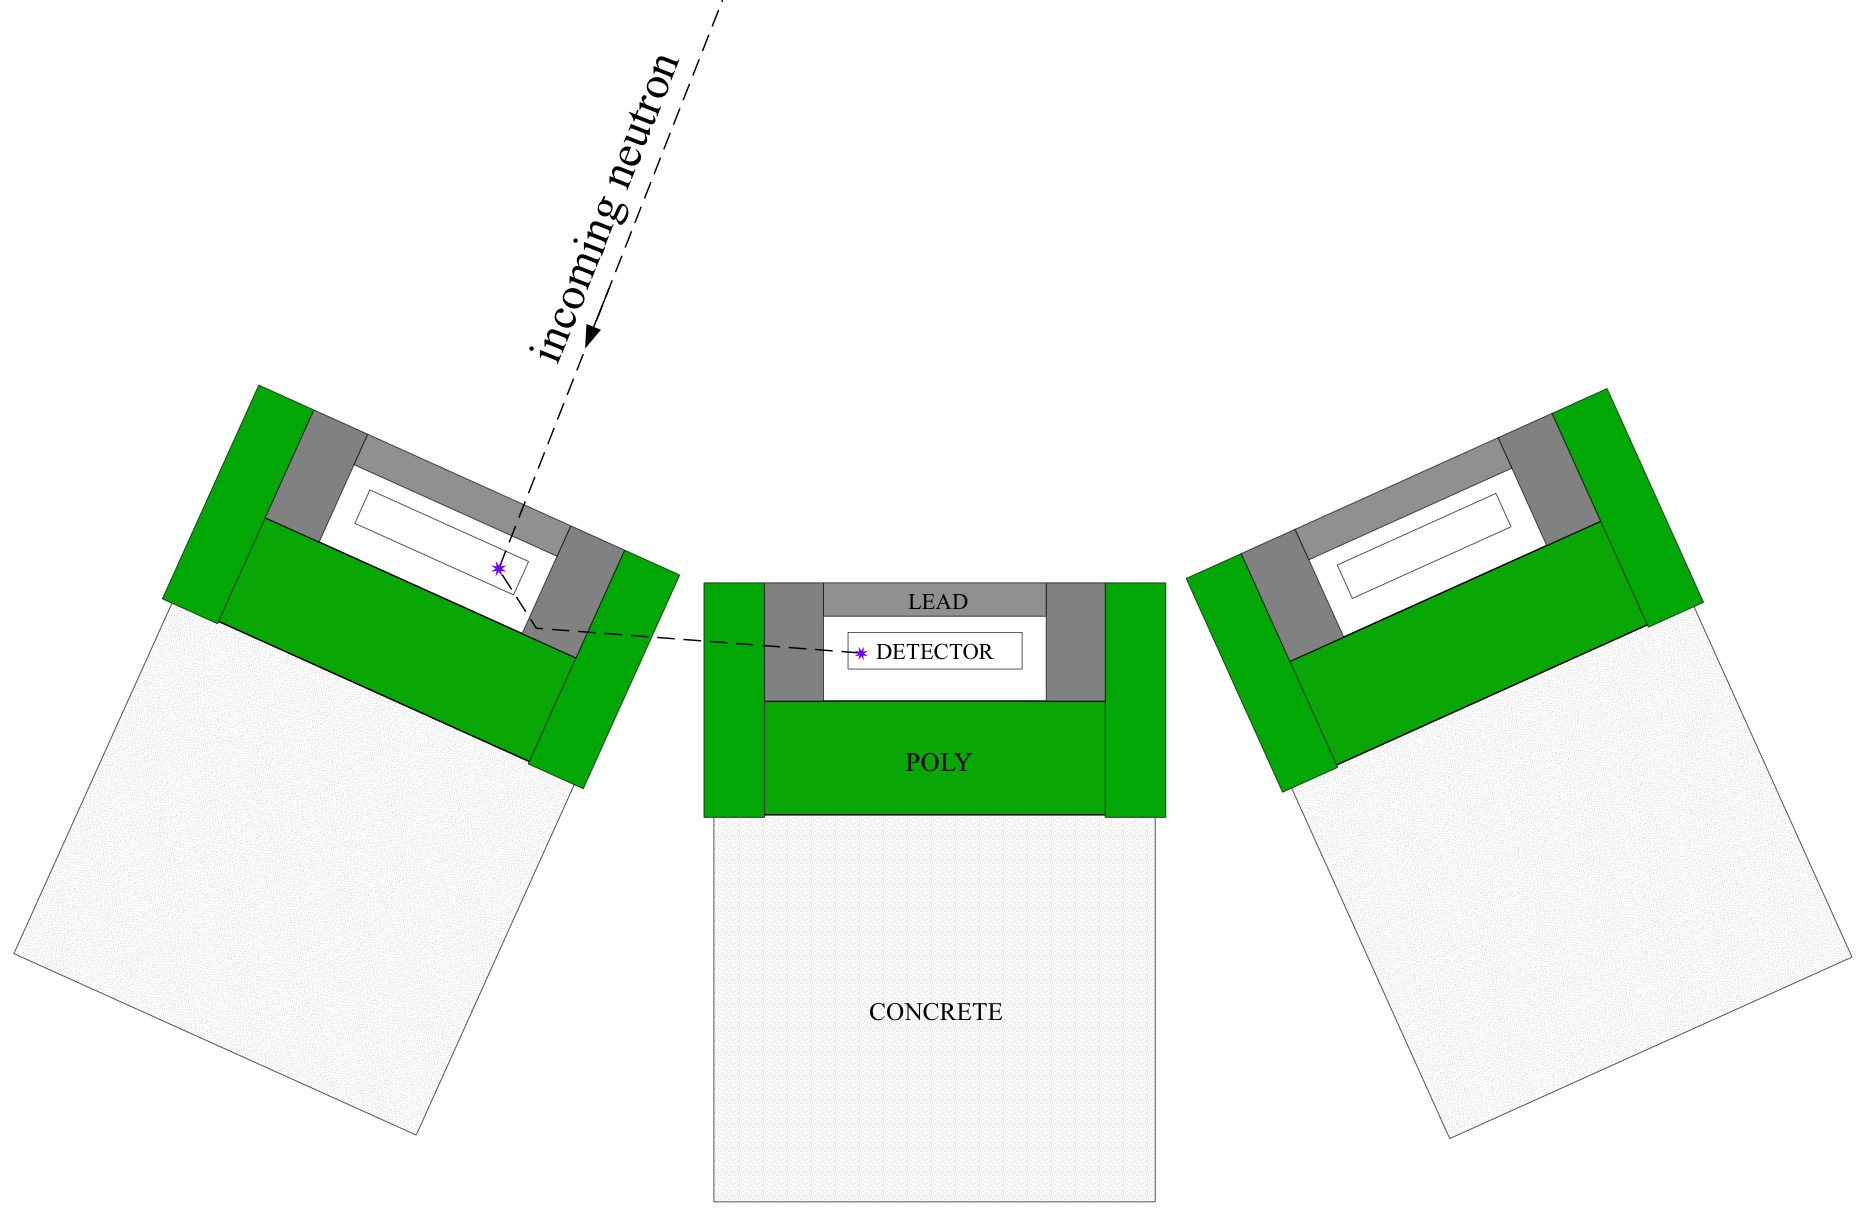
\includegraphics[width = 0.95\textwidth]{Content/Errors/CrossTalkExample.png}
    \caption{A hypothetical example of a neutron cross-talk event.
An incoming neutron is detected and then scatters from some lead shielding nearby, which changes its direction of travel such that it enters a second detector where it is detected a second time.
The scattering of a neutron from an intermediate nucleus, in this example a lead nucleus, is kinematically required in order for cross-talk to occur in this experiment.}
    \label{fig:CrossTalkExample}
\end{figure}

\section{Simulation of Detector Cross-talk}
A simulation was performed to ensure that the detector shielding effectively reduced cross-talk to negligible levels.
The simulation included all scintillators and their shielding, supporting structures, and the concrete walls surrounding the experimental cell.
MCNP-PoliMi's built-in $^{252}$Cf spontaneous fission source was used, which emits neutrons with the correct correlations and multiplicities.
Detector response was modeled using a program included with the MCNP-PoliMi distribution called MPPost~\cite{MPPost}.
The model is based on the electron equivalent light output (MeVee) produced by particles as they undergo collisions with carbon and hydrogen within organic plastic scintillators.
A minimum deposited energy of 0.4 MeV ( 0.05 MeVee for neutrons) was assumed for detectable particles, which was chosen because the neutron detection system showed a sharp decline in detection rates for neutrons below 0.4 MeV.
For neutron collisions with hydrogen, the light output in MeVee, $L$, is calculated by the following empirically derived formula
\begin{displaymath}
L = 0.0364 E_n^2 +  0.125 E_n
\end{displaymath}
where $E_n$ is equal to the loss in the kinetic energy of the neutron due to the collision.
Neutron interactions with carbon are assumed to generate a small light output of
\begin{displaymath}
L = 0.02 E_n
\end{displaymath}
As seen in Fig.~\ref{fig:Cf252MCNPVsEXP}, this model of the detection process produces a ToF spectrum that is in good agreement with the measurement.
\begin{figure}
    \centering
    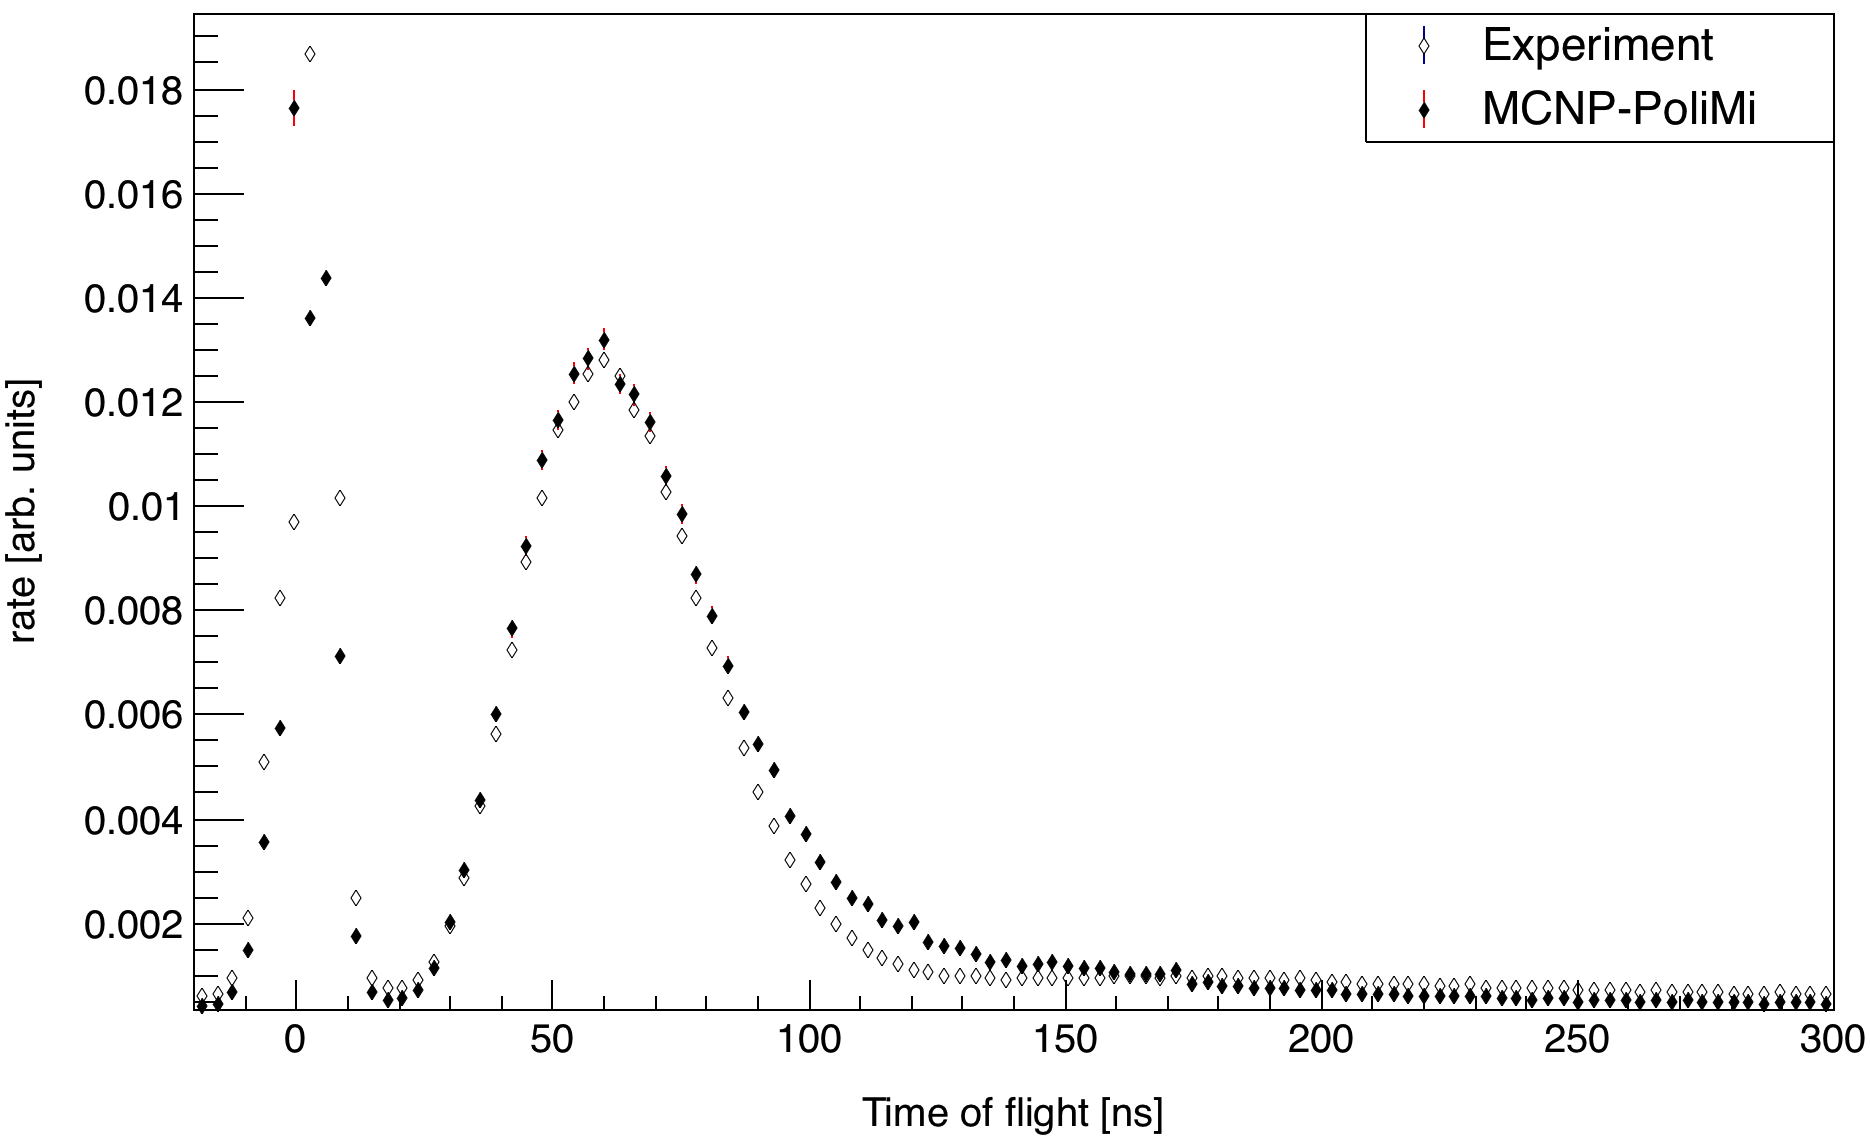
\includegraphics[width = 0.9\textwidth]{Content/Errors/Cf252MCNPVsEXP.png}
    \caption{Measured \emph{versus} simulated ToF spectrum of a $^{252}$Cf spontaneous fission source. 
    The simulation also used a detector response model based on ref~\cite{MPPost}}
    \label{fig:Cf252MCNPVsEXP}
\end{figure}

The simulation was initially performed with 5 cm of lead shielding placed behind the scintillators, and the number of cross-talk events accounted for 11\% of the total coincident neutron events.
The amount of cross-talk fell to 3\% if polyethylene was used instead of lead, which motivated the placement of 10~cm of polyethylene behind the detectors during construction.
Figure~\ref{fig:CrosstalkVScoincidence} shows the distribution of cross-talk events and true two-neutron coincidences as a function of reconstructed opening angle.
It is worth noting that, according to the simulation, the effect of cross-talk is not only small, but is also distributed over a wide range of angles rather than being concentrated around $\theta_{nn}=0$.
Angles greater than 125 degrees are not shown in Fig.~\ref{fig:CrosstalkVScoincidence}, because these cross-talk events can be readily identified in analysis by the large amount of time required for a neutron to travel the required distances.
\begin{figure}
    \centering
    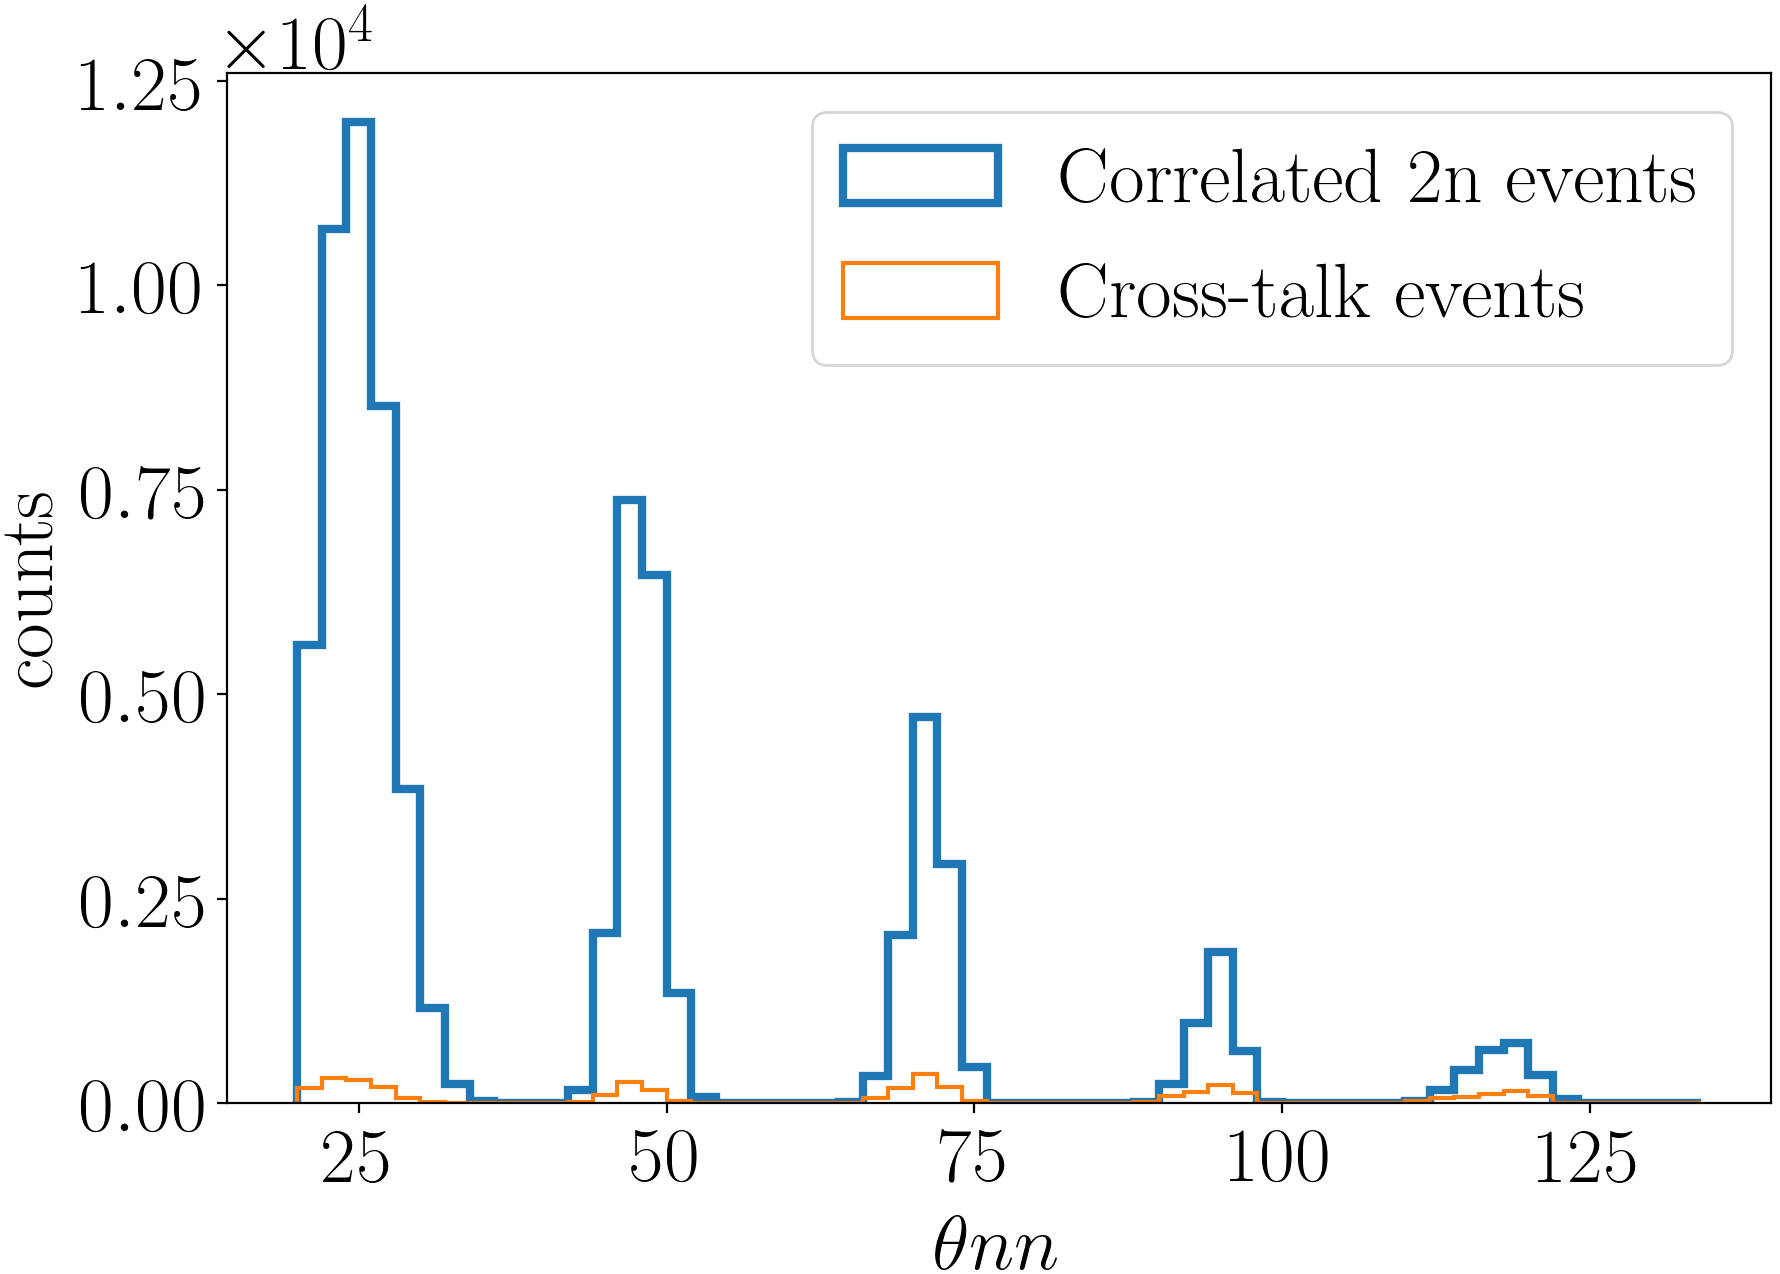
\includegraphics[width = 0.95\textwidth]{Content/Errors/CrosstalkVScoincidence.png}
    \caption{
    MCNP-PoLiMi simulation of the number of cross-talk events \emph{versus} correlated two-neutron events as a function of reconstructed opening angle.
    Cross-talk accounted for 3\% of total events.
    In this work, cross-talk does not occur primarily at small angles, but is instead spread out over a wide range of angles.
    }
    \label{fig:CrosstalkVScoincidence}
\end{figure}

\section{Neutron Scattering within Target}
\label{subsection:Elastic_scattering}
A potential source of error in opening angle measurements is the scattering of neutrons within the fission target.
This is a cause for concern, because when a neutron scatters from a heavy nucleons, such as $^{238}$U, is very likely to be deflected at a large angle, causing two-neutron opening angles that are not reflective of the opening angle immediately after fission.
Furthermore, because the target used in this work has the shape of a thin strip, it is more likely that neutrons emitted along the wider axis (2~cm) of the strip undergo a scattering event than it is for those emitted along the thinest axis (0.05~cm).
As a result, detectors that are located collinear to the widest axis of the target will see relatively fewer neutrons due to increased scattering. 
This bias is removed by slowly rotating the target about the vertical axis during data acquisition.
Because the subject of this measurement is fundamentally a statistical process, useful interpretations of the data are average rates taken over many events.
Thus, by rotating the target, cylindrical symmetry is preserved in the average, producing a result equivalent to that if a cylindrical target were used.

The target's dimensions are small enough that the rate of photon absorption, and thus photo-neutron production, is virtually uniform throughout the entire target volume.
MCNP-PoLiMi was used to simulate fission neutrons from the SF of $^{252}$Cf at locations distributed uniformly throughout the target volume.
The probability that at least one neutron out of a pair of two scatters before exiting the target was calculated from the simulation.
For the target used in this work, the result indicated that 6\% of two-neutron opening angles were perturbed due to scattering.

The rate of elastic scattering is also affected by the shape of the target.
A thin strip is the ideal target shape regarding the rate of neutron elastic scattering per unit of total target volume.
See Fig~\ref{fig:ElasticScatteringPlot} for the simulated elastic scattering rates for both thin strip and cylindrical shaped targets.
The simulation indicated that the rate of elastic scattering is about a factor of two times greater in cylindrical targets than in thin strip targets of the same volume and width-to-height ratio as the target used in this experiment.

\begin{figure}
    \centering
    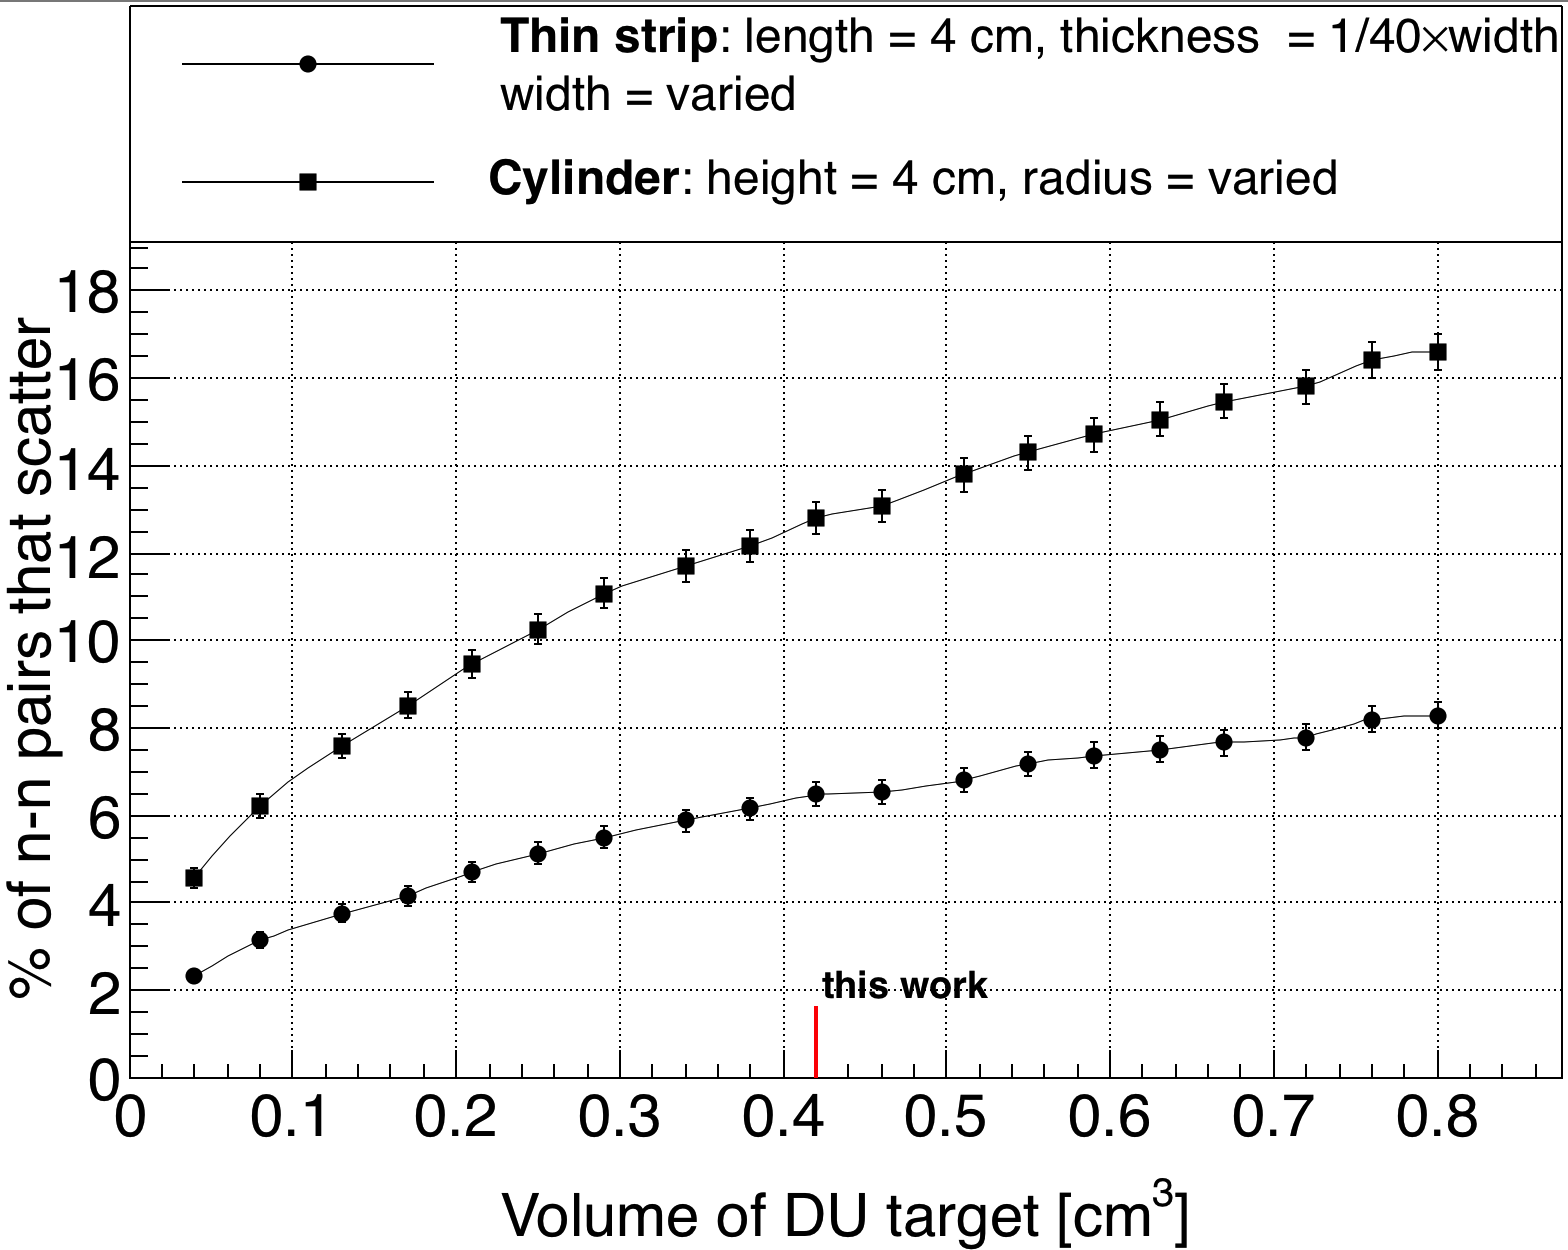
\includegraphics[width = 0.95\textwidth]{Content/Errors/ElasticScatteringPlot.png}
    \caption{
     Result of an MCNP simulation in which neutron-neutron pairs, with energies sampled from a typical watt fission spectrum, were generated uniformly throughout the volume of DU targets.
        The y-axis is the rate of opening angle contamination due to the scattering of, within the DU target in which they were produced, either one or both of a pair of neutrons.
    The lack of symmetry of a thin strip target can be removed by slowly rotating the target around the vertical axis during data acquisition, making it the optimal target geometry for the minimization of the rate of neutron scattering.
    The target used in this work had a length of 4~cm, a width of 2~cm, and a thickness of 0.05~cm.
    }
    \label{fig:ElasticScatteringPlot}
\end{figure}

Section~\ref{sec:anomaly} discusses the observation of an unexpected drop in correlation around 180$^{\circ}$ in our photofission of $^{238}$U measurement, as seen in Figs.~\ref{fig:DU(0)} through~\ref{fig:DU(1)}.
This motivated a simulation which examined whether this decrease in the correlation around 180$^{\circ}$ opening angles reflects the underlying physics of the fission process, or, arises from an artifact of the data analysis procedure.
In particular, note that throughout these measurements, the target was continuously rotated once per 8 seconds.
This means that for the determination of the uncorrelated opening angle distribution, the trajectories of the two neutrons were taken from two different pulses in which the target was at a different orientation for each of them.
Additionally, each of the neutrons likely originated from different regions of the target volume.
On the other hand, for the same-pulse, correlated neutron measurement, the target was in the same orientation and the two neutrons were generated at the same position in the target.
As such, we investigated whether these differences could cause this apparent decrease in the opening angle distribution.

Using the correlated $^{252}$Cf SF source built-in to MCNP-PoLiMi, the opening angle distribution of neutrons at the moment of emission can be compared to that of emitted neutrons after they have escaped the target.
Analysis of the simulation employs the same technique outlined in section~\ref{subsec:SPDPCancelation}, in which a correlated neutron distribution is divided by an uncorrelated neutron distribution.
In the case of the simulation, the correlated opening angle distribution is formed by pairing neutrons emitted during the same fission, and the uncorrected distribution by the pairing of neutrons emitted during different fissions.
The location of fission events were sampled uniformly throughout the targets volume.
In order to account for the effect of the rotating target on the trajectories of neutrons from different-pulses, the coordinate system was rotated accordingly for different fissions.
The conclusion was that a 0.05$\times$2$\times$4~cm$^3$ $^{238}$U target does not result in a significant departure from the true opening angle distribution due to neutron scattering.
Fig~\ref{fig:ElasticScatteringEffect} compares the two-neutron opening angle distribution at the moment of emission to that of neutrons once they have escaped the target.
\begin{figure}
    \centering
    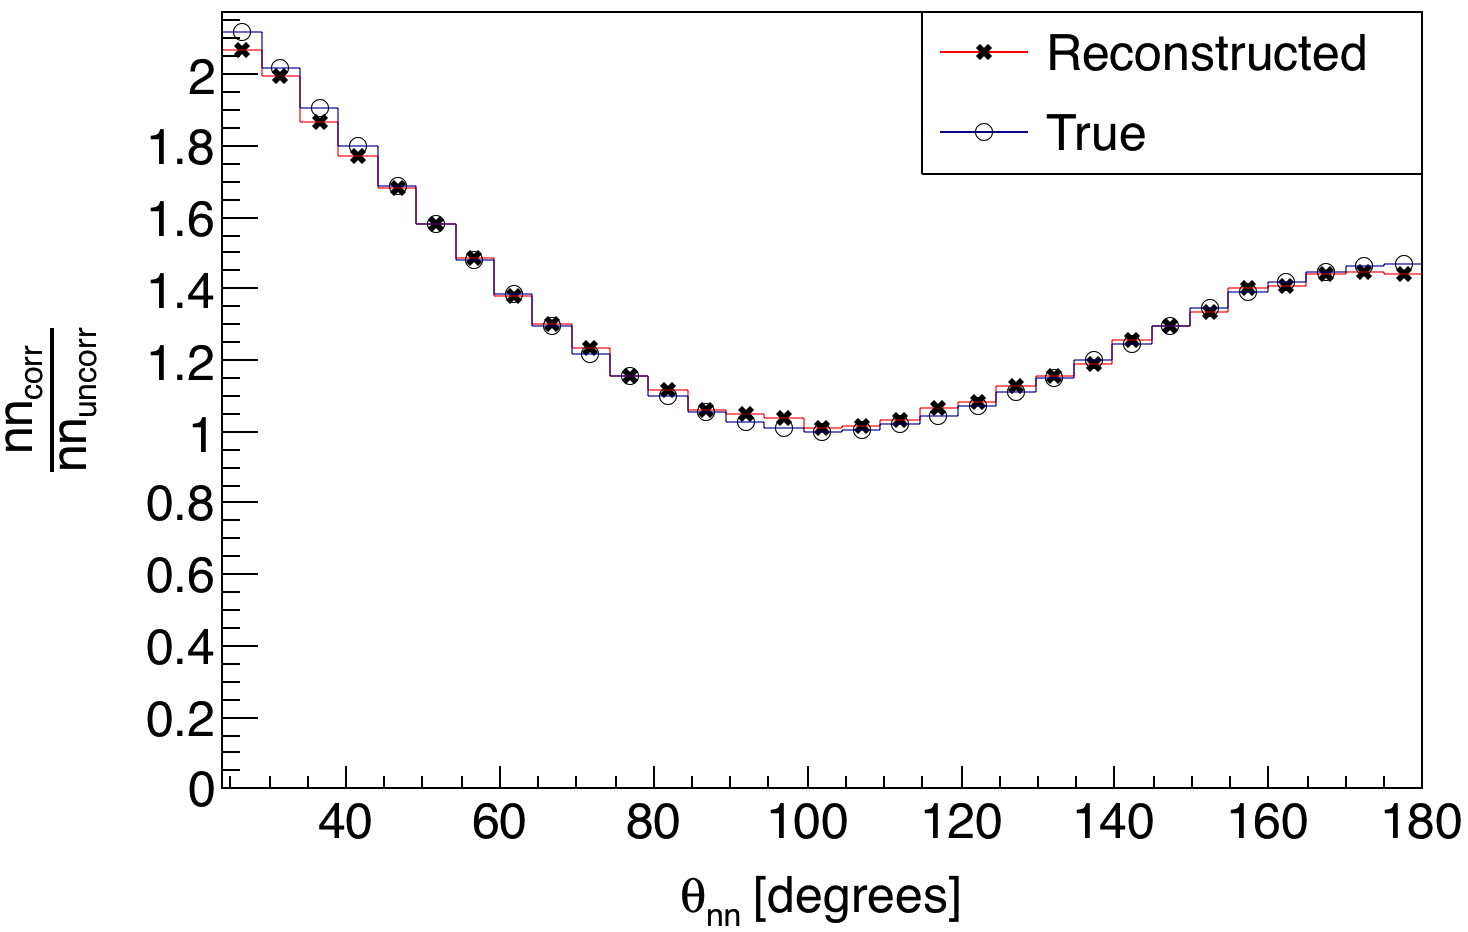
\includegraphics[width = 0.95\textwidth]{Content/Errors/EffectOfElasticScattering.png}
    \caption{MCNP-PoLiMi simulation of correlated $^{252}$Cf neutrons sampled uniformly throughout a 0.05$\times$2$\times$4~cm$^3$ $^{238}$U target.
    The purpose of this simulation was to rule out errors caused by the scattering of fission neutrons within the target.}
    \label{fig:ElasticScatteringEffect}
\end{figure}


